\documentclass[11pt,a4paper]{article}

% ------------------------------------------------------------------
% Packages
% ------------------------------------------------------------------
\usepackage[utf8]{inputenc}
\usepackage[T1]{fontenc}
\usepackage{lmodern}
\usepackage[margin=2.5cm]{geometry}
\usepackage{amsmath,amssymb,amsthm,mathtools}
\usepackage{booktabs}
\usepackage{graphicx}
\usepackage{xcolor}
\usepackage{listings}
\usepackage{algorithm}
\usepackage{algpseudocode}
\usepackage{caption}
\usepackage{subcaption}
\usepackage{pgfplots}
\usepgfplotslibrary{groupplots}
\pgfplotsset{compat=1.17}
\usepackage[colorlinks=true,linkcolor=blue!60!black,citecolor=blue!60!black,urlcolor=blue!60!black]{hyperref}
\usepackage{cleveref}

% ------------------------------------------------------------------
% Theorems
% ------------------------------------------------------------------
\newtheorem{lemma}{Lemma}
\newtheorem{proposition}{Proposition}[section]
\theoremstyle{remark}
\newtheorem{remark}{Remark}[section]

% ------------------------------------------------------------------
% Macros
% ------------------------------------------------------------------
\newcommand{\E}{\mathbb{E}}
\newcommand{\Q}{\mathbb{Q}}
\newcommand{\ind}{\mathbf{1}}
\newcommand{\dd}{\mathrm{d}}
\newcommand{\code}[1]{\texttt{#1}}
\newcommand{\todo}[1]{\textcolor{red}{\textbf{[TODO: #1]}}}

% Figures exported from Produits/Digitale/digital_pricer.ipynb into figures/.
% A framed placeholder is printed while a file is missing, so that the document always compiles.
\newcommand{\figfile}[2]{%
  \IfFileExists{figures/#1}{\includegraphics[width=#2]{figures/#1}}%
  {\fbox{\parbox[c][4cm][c]{#2}{\centering\small missing figure:\\ \texttt{figures/#1}}}}}

\lstset{basicstyle=\ttfamily\footnotesize, keywordstyle=\color{blue!70!black}, commentstyle=\color{gray},
        stringstyle=\color{teal}, frame=single, breaklines=true, language=Python, showstringspaces=false}

% ------------------------------------------------------------------
\title{Digital Options: Pricing, Greeks and Hedging}
\author{Elias Benguedda}
\date{October 2026}

\begin{document}
\emergencystretch=3em
\maketitle

\begin{abstract}
This paper studies the pricing and hedging of digital options on an equity
index, for the European, Bermudan and American exercise styles. Under the
Black--Scholes model we derive the closed-form prices and Greeks of European
cash-or-nothing and asset-or-nothing options, discuss the limits of delta
hedging and the static replication by call spreads, and prove that an American
cash digital is a one-touch option paid at hit, whose price follows from the
law of the first hitting time of a drifted Brownian motion. Since these
formulas ignore the smile and the volatility dynamics, the options are then
priced under a Heston model calibrated to the CAC~40 implied volatility surface
of 12 February 2025, by Monte Carlo simulation with the Longstaff--Schwartz
algorithm and a European digital control variate. The pricer is validated
against the Black--Scholes closed forms, and on the CAC~40 the early-exercise
right roughly doubles the price of the digital, with a call--put asymmetry
around the ``twice the European digital'' rule of thumb that is driven by the
skew.
\end{abstract}

\clearpage
\tableofcontents
\newpage

% ==================================================================
\section{Introduction}
\label{sec:intro}
% ==================================================================

\subsection{Motivation}

Digital options are liquid instruments, especially on FX markets, but they are
not vanilla products: their discontinuous payoff makes both their pricing and
their hedging delicate, and dedicated pricers are required.

\subsection{Outline}

Section~\ref{sec:products} describes the products and their model-free
properties, and derives the closed-form prices and Greeks of European digital
options under the Black--Scholes model, which serves as a benchmark.
Section~\ref{sec:data} presents the market data and the calibrated model used
in the rest of the paper. Section~\ref{sec:american} prices American digital options and
Section~\ref{sec:bermudan} Bermudan digital options.
Section~\ref{sec:greeks} studies their Greeks and Section~\ref{sec:hedging}
their hedging.

% ==================================================================
\section{Digital Options and European Pricing}
\label{sec:products}
% ==================================================================

Digital options, also called binary options, pay a fixed coupon when a trigger
event occurs. There are two kinds of digital options: cash-or-nothing (CON) and
asset-or-nothing (AON) options. Many underlyings are possible, such as a single
stock, an index or a basket. To keep the descriptions simple, we focus on the
call versions; the put versions follow by parity and are treated in the
associated notebook. In the following, $K$ denotes the trigger level (or
strike) and $Q$ the cash amount.

European digital options admit closed-form prices in the Black--Scholes
framework~\cite{BlackScholes1973,Merton1973}. We derive them together with the
description of the products; they serve as a benchmark for the stochastic
volatility results of Sections~\ref{sec:american} and~\ref{sec:bermudan}. The section ends with a
discussion of why these formulas are not sufficient for equity-index digitals.

% Figures use a logistic approximation of N(x) (max error ~1e-4),
% since pgfmath has no built-in normal CDF.

% ---------------------------------------------------------------------
\subsection{Model and Notation}
\label{subsec:bs-model}

Let $S_t$ denote the level of the underlying index. Under the risk-neutral
measure $\mathbb{Q}$, the index follows
\begin{equation}
  \mathrm{d}S_t = (r-q)\,S_t\,\mathrm{d}t + \sigma\,S_t\,\mathrm{d}W_t,
  \label{eq:bs-sde}
\end{equation}
where $r$ is the constant risk-free rate, $q$ the continuous dividend yield,
$\sigma$ the constant volatility and $W$ a standard Brownian motion. We write
$\tau = T-t$ for the time to maturity, $\nu = r - q - \tfrac{1}{2}\sigma^2$ for
the drift of $\ln S_t$, and
\begin{equation}
  d_1 = \frac{\ln(S_t/K) + \left(r - q + \tfrac{1}{2}\sigma^2\right)\tau}{\sigma\sqrt{\tau}},
  \qquad
  d_2 = d_1 - \sigma\sqrt{\tau}.
  \label{eq:d1d2}
\end{equation}
$N(\cdot)$ and $n(\cdot)$ denote the standard normal cumulative distribution
and density functions. Two probabilities appear throughout this section:
\begin{equation}
  \mathbb{Q}\left(S_T \geq K \mid \mathcal{F}_t\right) = N(d_2),
  \qquad
  \mathbb{Q}^S\left(S_T \geq K \mid \mathcal{F}_t\right) = N(d_1),
  \label{eq:probas}
\end{equation}
where $\mathbb{Q}^S$ is the share measure, defined by
\begin{equation}
  \left.\frac{\mathrm{d}\mathbb{Q}^S}{\mathrm{d}\mathbb{Q}}\right|_{\mathcal{F}_T}
  = \frac{S_T\, e^{-(r-q)T}}{S_0}.
\end{equation}

% ---------------------------------------------------------------------
\subsection{Cash-or-Nothing Options}
\label{subsec:con}

The European CON call is the simplest digital option. It pays the cash amount
$Q$ at maturity if the underlying finishes above the strike
(Figure~\ref{fig:payoff-con}):
\begin{equation}
  \mathrm{CON}_T = Q\,\ind_{\{S_T \geq K\}}.
  \label{eq:con-payoff}
\end{equation}
The CON put pays $Q\,\ind_{\{S_T < K\}}$ instead.

\begin{figure}[htbp]
\centering
\begin{tikzpicture}
\begin{axis}[
    axis lines=middle,
    xlabel={$S_T$}, ylabel={Payoff},
    xmin=0, xmax=10, ymin=0, ymax=6,
    xtick={4}, xticklabels={$K$},
    ytick={3}, yticklabels={$Q$},
    width=9cm, height=7cm,
    every axis x label/.style={at={(ticklabel* cs:1)}, anchor=west},
    every axis y label/.style={at={(ticklabel* cs:1)}, anchor=south},
]
    % Zero payoff below K
    \addplot[very thick, blue, domain=0:4] {0};
    % Payoff Q above K
    \addplot[very thick, blue, domain=4:9.5] {3};
    % Jump at K
    \draw[dashed, gray] (axis cs:4,0) -- (axis cs:4,3);
    \fill[blue] (axis cs:4,3) circle (2.5pt);
    \draw[blue, fill=white] (axis cs:4,0) circle (2.5pt);
\end{axis}
\end{tikzpicture}
\caption{Payoff of a European cash-or-nothing call.}
\label{fig:payoff-con}
\end{figure}

The price of a CON option is the discounted risk-neutral probability of
finishing in the money:
\begin{align}
  D^{c}(S_t,K,\tau) &= e^{-r\tau}\,\mathbb{E}^{\mathbb{Q}}\!\left[Q\,\mathbf{1}_{\{S_T \geq K\}} \mid \mathcal{F}_t\right]
                     = Q\,e^{-r\tau}\,N(d_2), \label{eq:cash-call}\\
  D^{p}(S_t,K,\tau) &= Q\,e^{-r\tau}\,N(-d_2). \label{eq:cash-put}
\end{align}

% ---------------------------------------------------------------------
\subsection{Asset-or-Nothing Options}
\label{subsec:aon}

The European AON call pays the value of the underlying at maturity if this
value is above the strike (Figure~\ref{fig:payoff-aon}):
\begin{equation}
  \mathrm{AON}_T = S_T\,\ind_{\{S_T \geq K\}}.
  \label{eq:aon-payoff}
\end{equation}
The AON put pays $S_T\,\ind_{\{S_T < K\}}$ instead.

\begin{figure}[htbp]
\centering
\begin{tikzpicture}
\begin{axis}[
    axis lines=middle,
    xlabel={$S_T$}, ylabel={Payoff},
    xmin=0, xmax=10, ymin=0, ymax=10,
    xtick={4}, xticklabels={$K$},
    ytick={4}, yticklabels={$K$},
    width=9cm, height=7cm,
    every axis x label/.style={at={(ticklabel* cs:1)}, anchor=west},
    every axis y label/.style={at={(ticklabel* cs:1)}, anchor=south},
]
    % Zero payoff below K
    \addplot[very thick, blue, domain=0:4] {0};
    % Payoff S_T above K
    \addplot[very thick, blue, domain=4:9.5] {x};
    % Jump at K
    \draw[dashed, gray] (axis cs:4,0) -- (axis cs:4,4);
    \fill[blue] (axis cs:4,4) circle (2.5pt);
    \draw[blue, fill=white] (axis cs:4,0) circle (2.5pt);
\end{axis}
\end{tikzpicture}
\caption{Payoff of a European asset-or-nothing call.}
\label{fig:payoff-aon}
\end{figure}

Changing numeraire to the share measure gives
\begin{align}
  A^{c}(S_t,K,\tau) &= e^{-r\tau}\,\mathbb{E}^{\mathbb{Q}}\!\left[S_T\,\mathbf{1}_{\{S_T \geq K\}} \mid \mathcal{F}_t\right]
                     = S_t\,e^{-q\tau}\,N(d_1), \label{eq:asset-call}\\
  A^{p}(S_t,K,\tau) &= S_t\,e^{-q\tau}\,N(-d_1). \label{eq:asset-put}
\end{align}

% ---------------------------------------------------------------------
\subsection{Parity Relations and Static Decomposition}

Since the call and put payoffs sum to a constant, the following parity
relations hold in any arbitrage-free model:
\begin{equation}
  D^{c} + D^{p} = Q\,e^{-r\tau},
  \qquad
  A^{c} + A^{p} = S_t\,e^{-q\tau}.
  \label{eq:digital-parity}
\end{equation}
Moreover, the payoff of a vanilla call decomposes into digital payoffs:
\begin{equation}
  (S_T - K)^+ = S_T\,\ind_{\{S_T \geq K\}} - K\,\ind_{\{S_T \geq K\}}.
\end{equation}
By absence of arbitrage, a vanilla call is therefore worth an asset-or-nothing
call minus $K$ cash-or-nothing calls with $Q=1$, in any model. Under
Black--Scholes,
\begin{equation}
  C(S_t,K,\tau) = A^{c}(S_t,K,\tau) - K\,D^{c}(S_t,K,\tau)
               = S_t\,e^{-q\tau}N(d_1) - K\,e^{-r\tau}N(d_2),
  \label{eq:vanilla-decomposition}
\end{equation}
which recovers the Black--Scholes formula. Digital options are therefore the
elementary building blocks of vanilla options.

% ---------------------------------------------------------------------
\subsection{Replication by Call Spreads and the Role of the Smile}
\label{subsec:call-spread}

A digital option can be seen as the limit of a call spread~\cite{Bouzoubaa2010}.
Consider a call spread with strikes $K-\epsilon$ and $K$, and a
digital call struck at $K$ paying $Q=1$. Then
\begin{equation}
  \text{Digital}(K)
  = \lim_{\epsilon \to 0} \frac{1}{\epsilon}
    \bigl( \text{Call}(K-\epsilon) - \text{Call}(K) \bigr)
  = -\frac{\partial\, \text{Call}(K)}{\partial K}.
  \label{eq:call-spread-limit}
\end{equation}
Figure~\ref{fig:digital-callspread} illustrates the convergence of the call
spread payoffs to the digital payoff.

\begin{figure}[htbp]
\centering
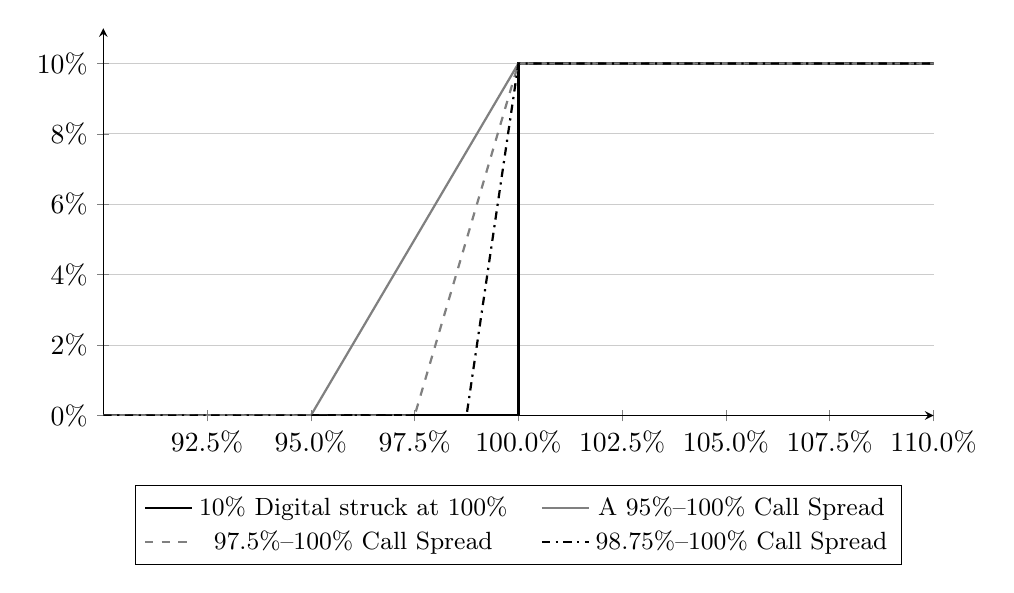
\begin{tikzpicture}
\begin{axis}[
    width=\textwidth, height=6.5cm,
    xmin=90, xmax=110, ymin=0, ymax=11,
    xtick={92.5,95,97.5,100,102.5,105,107.5,110},
    ytick={0,2,4,6,8,10},
    xticklabel={\pgfmathprintnumber[fixed,fixed zerofill,precision=1]{\tick}\%},
    yticklabel={\pgfmathprintnumber{\tick}\%},
    ymajorgrids=true,
    grid style={gray!40},
    axis x line=bottom, axis y line=left,
    legend style={
        at={(0.5,-0.18)}, anchor=north,
        legend columns=2, font=\small,
        /tikz/every even column/.append style={column sep=1em}
    },
]
    % 10% digital struck at 100%
    \addplot[black, thick] coordinates {(90,0) (100,0) (100,10) (110,10)};
    \addlegendentry{10\% Digital struck at 100\%}

    % 95%--105% call spread
    \addplot[gray, thick] coordinates {(90,0) (95,0) (100,10) (110,10)};
    \addlegendentry{A 95\%--100\% Call Spread}

    % 2 x 97.5%--102.5% call spread
    \addplot[gray, thick, dashed] coordinates {(90,0) (97.5,0) (100,10) (110,10)};
    \addlegendentry{97.5\%--100\% Call Spread}

    % 4 x 98.75%--101.25% call spread
    \addplot[black, thick, dash dot] coordinates {(90,0) (98.75,0) (100,10) (110,10)};
    \addlegendentry{98.75\%--100\% Call Spread}
\end{axis}
\end{tikzpicture}
\caption{A 10\% digital and three call spreads with different strikes. The closer the
call spread strikes are to the digital strike, the closer the payoff.}
\label{fig:digital-callspread}
\end{figure}

With a flat
volatility, differentiating the Black--Scholes formula gives
$-\partial C/\partial K = e^{-r\tau}N(d_2)$, consistent
with~\eqref{eq:cash-call}. When the market quotes a strike-dependent implied
volatility $\sigma(K)$, the call price is
$C^{\mathrm{mkt}}(K) = C^{\mathrm{BS}}\bigl(K,\sigma(K)\bigr)$ and the chain rule
yields
\begin{equation}
  D^{c,\mathrm{mkt}}(K)
  = e^{-r\tau}N(d_2) - \mathcal{V}^{\mathrm{BS}}(K)\,\frac{\partial \sigma}{\partial K},
  \qquad
  \mathcal{V}^{\mathrm{BS}}(K) = S_t\,e^{-q\tau}\,n(d_1)\sqrt{\tau},
  \label{eq:smile-correction}
\end{equation}
where $d_2$ is evaluated at $\sigma(K)$ and $\mathcal{V}^{\mathrm{BS}}$ is the
vega of the vanilla call. Equity indices exhibit a negative skew
($\partial\sigma/\partial K < 0$), so the market price of a digital call is
\emph{higher} than its Black--Scholes price computed with $\sigma(K)$, and the
market price of a digital put is correspondingly lower. Pricing a digital with
a single volatility therefore ignores a first-order effect of the smile.
We observe that for the pricing of European digital option, we don't need any volatility model, as long as we have the volatility of the strike price.


% ---------------------------------------------------------------------
\subsection{Greeks}
\label{subsubsec:bs-greeks}

For a cash-or-nothing call with $Q=1$, differentiating~\eqref{eq:cash-call}
gives
\begin{align}
  \Delta^{c} &= \frac{\partial D^{c}}{\partial S}
              = \frac{e^{-r\tau}\,n(d_2)}{S\,\sigma\sqrt{\tau}}, \label{eq:digital-delta}\\
  \Gamma^{c} &= \frac{\partial^2 D^{c}}{\partial S^2}
              = -\frac{e^{-r\tau}\,n(d_2)\,d_1}{S^2\,\sigma^2\,\tau}, \label{eq:digital-gamma}\\
  \mathcal{V}^{c} &= \frac{\partial D^{c}}{\partial \sigma}
              = -\frac{e^{-r\tau}\,n(d_2)\,d_1}{\sigma}. \label{eq:digital-vega}
\end{align}
As for vanilla options, vega and gamma are linked by
$\mathcal{V}^{c} = \sigma\,S^2\,\tau\,\Gamma^{c}$. By the parity
relation~\eqref{eq:digital-parity}, the Greeks of the cash-or-nothing put are
the opposite of those of the call.

Three features distinguish these Greeks from those of a vanilla option
(Figures~\ref{fig:bs-digital-price} to~\ref{fig:bs-digital-vega}):
\begin{itemize}
  \item the delta is bell-shaped around the strike and, as $\tau \to 0$,
        converges to a Dirac mass at $K$: close to maturity, the hedge ratio
        becomes unbounded for an at-the-money digital;
  \item gamma and vega change sign at $d_1 = 0$, i.e.\ at
        $S = K e^{-(r-q+\sigma^2/2)\tau}$: they are positive when the option
        is out of the money and negative when it is in the money;
  \item consequently, a digital option is not a monotone bet on volatility:
        an increase in volatility raises the price of an out-of-the-money
        digital and lowers the price of an in-the-money one.
\end{itemize}
A systematic comparison with the Greeks obtained under stochastic volatility
is carried out in Section~\ref{sec:greeks}.

% --- Figure: price -----------------------------------------------------
\begin{figure}[htbp]
\centering
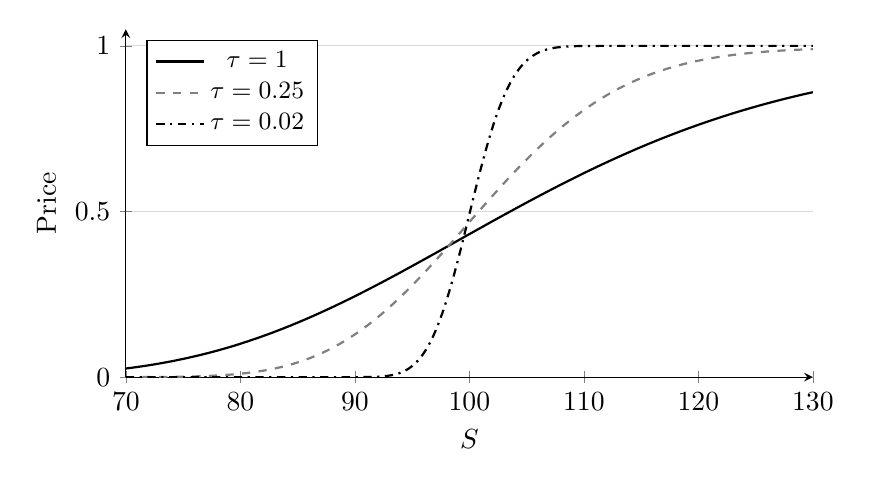
\begin{tikzpicture}
\begin{axis}[
    width=0.85\textwidth, height=6cm,
    xmin=70, xmax=130, ymin=0, ymax=1.05,
    xlabel={$S$}, ylabel={Price},
    ymajorgrids=true, grid style={gray!30},
    axis x line=bottom, axis y line=left,
    legend pos=north west, legend style={font=\small},
    samples=200,
    % Parameters: K = 100, r = 2%, q = 3%, sigma = 20%
    declare function={
      Ncdf(\x) = 1/(1+exp(-0.07056*\x*\x*\x - 1.5976*\x));
      dtwo(\s,\t) = (ln(\s/100) - 0.03*\t)/(0.2*sqrt(\t));
    },
]
  \addplot[black, thick, domain=70:130] {exp(-0.02*1)*Ncdf(dtwo(x,1))};
  \addlegendentry{$\tau = 1$}
  \addplot[gray, thick, dashed, domain=70:130] {exp(-0.02*0.25)*Ncdf(dtwo(x,0.25))};
  \addlegendentry{$\tau = 0.25$}
  \addplot[black, thick, dash dot, domain=70:130] {exp(-0.02*0.02)*Ncdf(dtwo(x,0.02))};
  \addlegendentry{$\tau = 0.02$}
\end{axis}
\end{tikzpicture}
\caption{Black--Scholes price of a cash-or-nothing call ($Q=1$) as a function
of the spot, for several maturities ($K=100$, $r=2\%$, $q=3\%$,
$\sigma=20\%$).}
\label{fig:bs-digital-price}
\end{figure}

% --- Figure: delta -----------------------------------------------------
\begin{figure}[htbp]
\centering
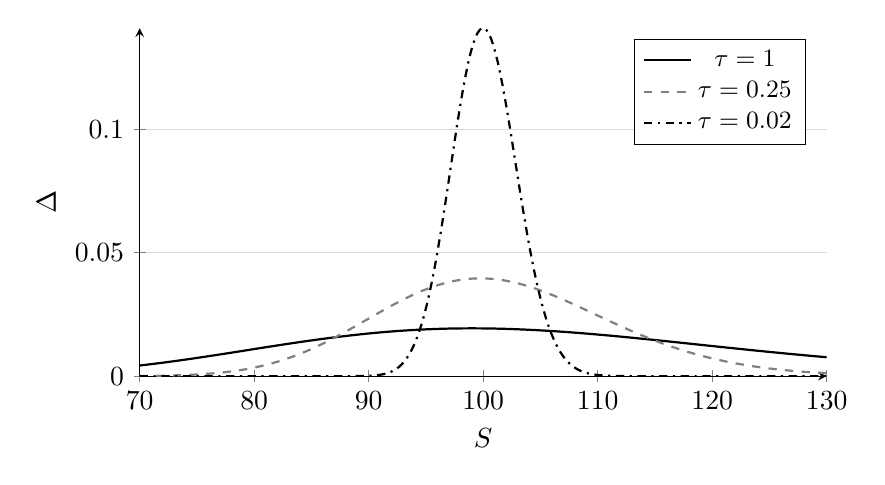
\begin{tikzpicture}
\begin{axis}[
    width=0.85\textwidth, height=6cm,
    xmin=70, xmax=130, ymin=0,
    xlabel={$S$}, ylabel={$\Delta$},
    ymajorgrids=true, grid style={gray!30},
    axis x line=bottom, axis y line=left,
    legend pos=north east, legend style={font=\small},
    scaled y ticks=false,
    yticklabel style={/pgf/number format/fixed, /pgf/number format/precision=2},
    samples=300,
    % Parameters: K = 100, r = 2%, q = 3%, sigma = 20%
    declare function={
      dtwo(\s,\t) = (ln(\s/100) - 0.03*\t)/(0.2*sqrt(\t));
      delta(\s,\t) = exp(-0.02*\t)*exp(-0.5*dtwo(\s,\t)*dtwo(\s,\t))
                     /(sqrt(2*pi)*\s*0.2*sqrt(\t));
    },
]
  \addplot[black, thick, domain=70:130] {delta(x,1)};
  \addlegendentry{$\tau = 1$}
  \addplot[gray, thick, dashed, domain=70:130] {delta(x,0.25)};
  \addlegendentry{$\tau = 0.25$}
  \addplot[black, thick, dash dot, domain=70:130] {delta(x,0.02)};
  \addlegendentry{$\tau = 0.02$}
\end{axis}
\end{tikzpicture}
\caption{Black--Scholes delta of a cash-or-nothing call ($Q=1$). The delta
concentrates around the strike as maturity approaches.}
\label{fig:bs-digital-delta}
\end{figure}

Let's note that for a digital call, $\Delta$ goes to the infinity at strike price, because the derivative of the payoff in respect to the spot price goes vertical.

% --- Figure: gamma -----------------------------------------------------
\begin{figure}[htbp]
\centering
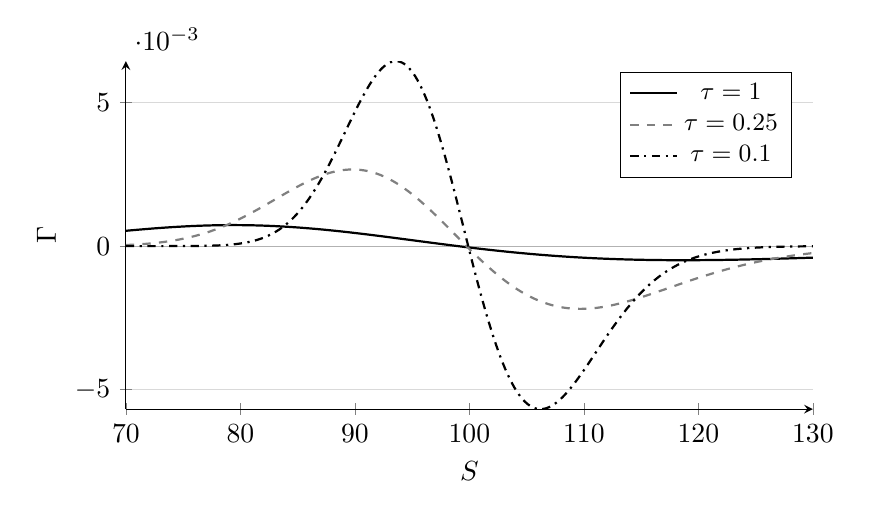
\begin{tikzpicture}
\begin{axis}[
    width=0.85\textwidth, height=6cm,
    xmin=70, xmax=130,
    xlabel={$S$}, ylabel={$\Gamma$},
    ymajorgrids=true, grid style={gray!30},
    axis x line=bottom, axis y line=left,
    legend pos=north east, legend style={font=\small},
    samples=300,
    % Parameters: K = 100, r = 2%, q = 3%, sigma = 20%
    declare function={
      dtwo(\s,\t) = (ln(\s/100) - 0.03*\t)/(0.2*sqrt(\t));
      done(\s,\t) = dtwo(\s,\t) + 0.2*sqrt(\t);
      gam(\s,\t)  = -exp(-0.02*\t)*exp(-0.5*dtwo(\s,\t)*dtwo(\s,\t))*done(\s,\t)
                    /(sqrt(2*pi)*\s*\s*0.04*\t);
    },
]
  \addplot[gray!60, thin, domain=70:130, forget plot] {0};
  \addplot[black, thick, domain=70:130] {gam(x,1)};
  \addlegendentry{$\tau = 1$}
  \addplot[gray, thick, dashed, domain=70:130] {gam(x,0.25)};
  \addlegendentry{$\tau = 0.25$}
  \addplot[black, thick, dash dot, domain=70:130] {gam(x,0.1)};
  \addlegendentry{$\tau = 0.1$}
\end{axis}
\end{tikzpicture}
\caption{Black--Scholes gamma of a cash-or-nothing call ($Q=1$, $K=100$,
$r=2\%$, $q=3\%$, $\sigma=20\%$). Gamma is positive out of the money, negative
in the money, and its magnitude grows like $1/\tau$ near the strike; the
shortest maturity is set to $\tau=0.1$ to keep the three curves readable.}
\label{fig:bs-digital-gamma}
\end{figure}


Let's also note that $\gamma$ also goes to the infinity because of the dicontinuity of the $\Delta$.

% --- Figure: vega ------------------------------------------------------
\begin{figure}[htbp]
\centering
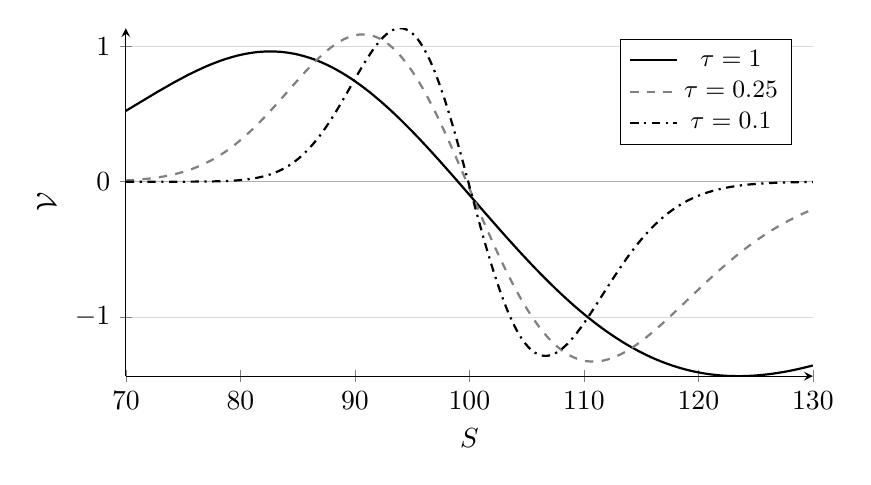
\begin{tikzpicture}
\begin{axis}[
    width=0.85\textwidth, height=6cm,
    xmin=70, xmax=130,
    xlabel={$S$}, ylabel={$\mathcal{V}$},
    ymajorgrids=true, grid style={gray!30},
    axis x line=bottom, axis y line=left,
    legend pos=north east, legend style={font=\small},
    samples=300,
    % Parameters: K = 100, r = 2%, q = 3%, sigma = 20%
    declare function={
      dtwo(\s,\t) = (ln(\s/100) - 0.03*\t)/(0.2*sqrt(\t));
      done(\s,\t) = dtwo(\s,\t) + 0.2*sqrt(\t);
      veg(\s,\t)  = -exp(-0.02*\t)*exp(-0.5*dtwo(\s,\t)*dtwo(\s,\t))*done(\s,\t)
                    /(sqrt(2*pi)*0.2);
    },
]
  \addplot[gray!60, thin, domain=70:130, forget plot] {0};
  \addplot[black, thick, domain=70:130] {veg(x,1)};
  \addlegendentry{$\tau = 1$}
  \addplot[gray, thick, dashed, domain=70:130] {veg(x,0.25)};
  \addlegendentry{$\tau = 0.25$}
  \addplot[black, thick, dash dot, domain=70:130] {veg(x,0.1)};
  \addlegendentry{$\tau = 0.1$}
\end{axis}
\end{tikzpicture}
\caption{Black--Scholes vega of a cash-or-nothing call ($Q=1$, $K=100$,
$r=2\%$, $q=3\%$, $\sigma=20\%$). Vega has the same sign pattern as gamma:
a rise in volatility helps the out-of-the-money digital and hurts the
in-the-money one.}
\label{fig:bs-digital-vega}
\end{figure}

\subsection{Hedging}

Unfortunately, we have some issues with this approach, we can wonder how to hedge a long call position on a digital regarding the dynamic of the greeks. Second point is which volatility are we taking to price this asset (because of course Black Scholes model does not reproduce the skew effect). A trader who rebalances his portfolio discretly once a day can't hedge the last decision because of the binary decision of the digital option.


Gamma plays another role, in a sens that it impacts significatively the tracking error $e_t$ of the delta-hedging, we have $de_t \approx O(\Gamma_t(\sigma_S^2-\sigma_{BS}^2)dt$


And here we use the replication technique with a call spread. Now the construction of the call spread depends of the liquidity of the two call strike options.


Considering a constant $\epsilon$ is a limitation because, as a seller, it overprices the digital option:

\begin{equation}
  \frac{N}{\epsilon} CallSpread(K- \epsilon) \approx N Digital(K)
\end{equation}

This approach also seems to be useless for the investor, because he would not need the bank in order to have a call spread.


Alternatively, this is why we need to consider dynamic hedging of the call spread position.


\subsection{Limits of dynamic delta hedging.}
In theory, the seller of a digital call can replicate the payoff by holding
$\Delta^{c}$ units of the underlying at all times. In practice, this strategy
breaks down as maturity approaches. From~\eqref{eq:digital-delta}
and~\eqref{eq:digital-gamma}, the delta grows like $1/(S\sigma\sqrt{\tau})$ and
the gamma like $1/(S^2\sigma^2\tau)$ when the spot is close to the strike, so
both diverge as $\tau \to 0$. Since the hedge must be rebalanced by
$\mathrm{d}\Delta \approx \Gamma\,\mathrm{d}S$ at each step, an exploding gamma
means that small market moves require very large trades in the underlying.
Transaction costs, which are proportional to the traded quantities, therefore
grow without bound, and the hedging error caused by discrete rebalancing grows
with gamma as well. Moreover, a jump or an overnight gap around the strike can
switch the payoff between $0$ and $Q$ before the hedge can be adjusted
(\emph{pin risk}). For an at-the-money digital close to expiry, the cost and the
residual risk of delta hedging thus become too large for the strategy to be
implemented.


\subsection{Static hedging with call spreads.}
The replication formula~\eqref{eq:call-spread-limit} suggests a static
alternative. Using two listed strikes $\epsilon$ apart, the seller of a digital
call buys $Q/\epsilon$ calls struck at $K-\epsilon$ and sells $Q/\epsilon$
calls struck at $K$. At maturity, this position pays
\begin{equation*}
  \frac{Q}{\epsilon}\Bigl[(S_T - K + \epsilon)^+ - (S_T - K)^+\Bigr]
  \;\geq\; Q\,\mathbf{1}_{\{S_T \geq K\}},
\end{equation*}
so the digital is over-hedged in every scenario, without any rebalancing and
without pin risk. The price of this protection is the small premium of the call
spread over the digital, which the seller passes on to the buyer by
\emph{shifting the strike}. The choice of $\epsilon$ is a trade-off: a smaller
spread reduces this premium but requires a larger notional of options, with
higher transaction costs and larger exposures on each leg. Finally, since the
call spread is built from market prices, it automatically incorporates the
smile correction~\eqref{eq:smile-correction} and does not rely on any model of
volatility dynamics. For these reasons, static replication with call spreads is
the standard way to hedge European digital options in practice.

% ---------------------------------------------------------------------
\subsection{Exercise Styles and Touch Options}

Both CON and AON options also exist in American and Bermudan versions, in which
the trigger is monitored not only at maturity but continuously, or on a
discrete set of dates, before maturity. Contracts typically specify a
monitoring of the trigger at each daily close. The coupon may then be paid
either when the trigger is hit or at maturity. As always for early-exercise
products, such options are harder to price because the exercise time is
unknown.

Path-dependent digitals come in several types:
\begin{enumerate}
  \item \textbf{One-touch:} pays if and only if the barrier is touched, either
        immediately or at maturity;
  \item \textbf{No-touch:} pays if and only if the barrier is never touched;
  \item \textbf{Double one-touch:} two barriers, pays if and only if either
        barrier is touched;
  \item \textbf{Double no-touch:} two barriers, pays if and only if neither
        barrier is touched.
\end{enumerate}
Their prices are derived in Sections~\ref{sec:american} and~\ref{sec:bermudan},
first under Black--Scholes and then under the Heston model.

% ---------------------------------------------------------------------
\subsection{Limitations of the Black--Scholes Framework}
\label{subsec:bs-limits}

The formulas above are exact under the assumptions of the model, but these
assumptions are particularly restrictive for digital options on an equity
index.

\begin{enumerate}
  \item \textbf{No smile.} The model uses a single volatility, whereas the
        market quotes a skewed implied volatility surface. As shown
        by~\eqref{eq:smile-correction}, the price of a European digital
        depends on the slope of the smile at the strike, which no choice of a
        single $\sigma$ can capture consistently across strikes.
  \item \textbf{No volatility dynamics.} American and Bermudan digitals depend
        on the whole path of the underlying. Their prices are determined not
        only by today's surface but by its future evolution (forward skew,
        volatility of volatility, spot--volatility correlation), which the
        Black--Scholes model fixes by assumption.
  \item \textbf{Hedging instability.} The unbounded delta and gamma near the
        strike at maturity make the theoretical delta hedge impossible to
        implement. In practice, digitals are hedged and priced conservatively
        with call spreads, as in~\eqref{eq:call-spread-limit}, at a cost that
        depends on the smile.
\end{enumerate}

These limitations motivate the stochastic volatility model presented in
Section~\ref{sec:data}, in which the spot--volatility correlation generates
a skew and the volatility of volatility governs the path-dependent effects.

\clearpage

% ==================================================================
\section{Market Data and Model}
\label{sec:data}
% ==================================================================

\subsection{Data}

As usual, the data used in this paper are available on my
website\footnote{\url{https://portfolio-eliasbenguedda.fr}}. We use CAC~40
option quotes of 12 February 2025 to build an implied volatility surface.

\subsection{Model}

We use the Heston model, previously calibrated to this
surface\footnote{\url{https://portfolio-eliasbenguedda.fr/projects/Heston.html}}.

% ==================================================================
\section{Pricing of American Digital Options}
\label{sec:american}
% ==================================================================

This section prices digital options that can be exercised at any time before
maturity. We first derive closed-form prices under the Black--Scholes model of
Section~\ref{subsec:bs-model}, which serve as benchmarks, and then price the
options under the Heston model calibrated in Section~\ref{sec:data}.

% ---------------------------------------------------------------------
\subsection{Optimal Exercise and Equivalence with One-Touch Options}

An American cash-or-nothing call allows its holder to exercise at any stopping
time $\theta \in [t,T]$ and to receive $Q$ provided $S_\theta \geq K$. Let
$\tau_K = \inf\{u \geq t : S_u \geq K\}$ be the first hitting time of the
strike.

\begin{proposition}
\label{prop:american-one-touch}
If $r \geq 0$ and $S_t < K$, the American cash-or-nothing call is equivalent
to a one-touch option with barrier $B = K$ paying $Q$ at the hitting time:
\begin{equation}
  V^{\mathrm{Am}}_t = Q\,\mathbb{E}^{\mathbb{Q}}\!\left[e^{-r(\tau_K - t)}\,\mathbf{1}_{\{\tau_K \leq T\}} \mid \mathcal{F}_t\right].
  \label{eq:american-one-touch}
\end{equation}
\end{proposition}

\begin{proof}
Any exercise strategy pays only at a time $\theta$ such that
$S_\theta \geq K$, hence $\theta \geq \tau_K$. Since $r \geq 0$,
$e^{-r(\theta-t)} \leq e^{-r(\tau_K-t)}$, so no strategy is worth more than
the right-hand side of~\eqref{eq:american-one-touch}. The strategy
$\theta = \tau_K$ attains this bound.
\end{proof}

\begin{remark}
When $r < 0$, as was the case for euro rates between 2015 and 2022, delaying
the payment becomes valuable and the equivalence no longer holds. The same
argument then only gives the bounds
$\mathrm{OT}^{\mathrm{hit}} \leq V^{\mathrm{Am}} \leq \mathrm{OT}^{\mathrm{exp}}$,
where $\mathrm{OT}^{\mathrm{hit}}$ and $\mathrm{OT}^{\mathrm{exp}}$ are the
one-touch options paying at the hitting time and at maturity respectively.
\end{remark}


\subsection{One-Touch pricing:}
\subsubsection{One-Touch Paying at Hit: Black Scholes Assumptions}
\label{subsec:one-touch-hit}

Let $\eta = -1$ for an upper barrier ($S_t < B$, one-touch call) and
$\eta = +1$ for a lower barrier ($S_t > B$, one-touch put), and define
\begin{equation}
  \mu = \frac{\nu}{\sigma^2},
  \qquad
  \lambda = \sqrt{\mu^2 + \frac{2r}{\sigma^2}},
  \qquad
  z = \frac{\ln(B/S_t)}{\sigma\sqrt{\tau}} + \lambda\,\sigma\sqrt{\tau}.
  \label{eq:ot-parameters}
\end{equation}

\begin{proposition}
\label{prop:one-touch-hit}
The price of a one-touch option paying $Q$ at the first hitting time
$\tau_B = \inf\{u \geq t : S_u = B\}$, if $\tau_B \leq T$,
is~\cite{ReinerRubinstein1991,Haug2007}
\begin{equation}
  \mathrm{OT}^{\mathrm{hit}}
  = Q\left[\left(\frac{B}{S_t}\right)^{\mu+\lambda} N(\eta z)
  + \left(\frac{B}{S_t}\right)^{\mu-\lambda} N\!\left(\eta z - 2\eta\lambda\sigma\sqrt{\tau}\right)\right].
  \label{eq:one-touch-hit}
\end{equation}
\end{proposition}

The proof relies on the law of the first hitting time of a Brownian motion
with drift, which we recall first.

\begin{lemma}[First hitting time of a drifted Brownian motion]
\label{lem:hitting-time}
Let $X_u = \nu u + \sigma W_u$ with $X_0 = 0$, let $b > 0$ and
$T_b = \inf\{u \geq 0 : X_u = b\}$. Then $T_b$ has density
\begin{equation}
  f_{\nu}(u) = \frac{b}{\sigma\sqrt{2\pi u^3}}
  \exp\!\left(-\frac{(b - \nu u)^2}{2\sigma^2 u}\right), \qquad u > 0,
  \label{eq:hitting-density}
\end{equation}
and distribution function
\begin{equation}
  \mathbb{P}(T_b \leq u)
  = N\!\left(\frac{\nu u - b}{\sigma\sqrt{u}}\right)
  + e^{2\nu b/\sigma^2}\, N\!\left(\frac{-b - \nu u}{\sigma\sqrt{u}}\right).
  \label{eq:hitting-cdf}
\end{equation}
\end{lemma}

\begin{proof}
\emph{Driftless case.} For $\nu = 0$, the reflection principle states that,
for $m > 0$,
\begin{equation*}
  \mathbb{P}\Bigl(\max_{s \leq u} W_s \geq m\Bigr) = 2\,\mathbb{P}(W_u \geq m):
\end{equation*}
reflecting a path about the level $m$ after its first passage yields a path
with the same law, by the symmetry of Brownian increments and the strong
Markov property. Hence $\mathbb{P}(T_b \leq u) = 2N\bigl(-b/(\sigma\sqrt{u})\bigr)$,
and differentiating in $u$ gives
$f_0(u) = \frac{b}{\sigma\sqrt{2\pi u^3}}\exp\bigl(-\frac{b^2}{2\sigma^2 u}\bigr)$.

\emph{General case.} Let $\mathbb{P}^0$ be a measure under which $X$ is a
driftless Brownian motion with volatility $\sigma$. By Girsanov's theorem, the
measure $\mathbb{P}^{\nu}$ under which $X$ has drift $\nu$ is given by
\begin{equation*}
  \left.\frac{\mathrm{d}\mathbb{P}^{\nu}}{\mathrm{d}\mathbb{P}^{0}}\right|_{\mathcal{F}_u}
  = \exp\!\left(\frac{\nu}{\sigma^2}X_u - \frac{\nu^2}{2\sigma^2}u\right).
\end{equation*}
On the event $\{T_b = u\}$ we have $X_u = b$, so by optional stopping the
density of $T_b$ under $\mathbb{P}^{\nu}$ is
\begin{equation*}
  f_{\nu}(u) = f_0(u)\, \exp\!\left(\frac{\nu b}{\sigma^2} - \frac{\nu^2 u}{2\sigma^2}\right)
  = \frac{b}{\sigma\sqrt{2\pi u^3}}
    \exp\!\left(-\frac{b^2 - 2\nu b u + \nu^2 u^2}{2\sigma^2 u}\right),
\end{equation*}
which is~\eqref{eq:hitting-density}. Formula~\eqref{eq:hitting-cdf} follows by
integrating $f_{\nu}$, as can be checked by differentiating its right-hand
side~\cite{Shreve2004}.
\end{proof}

\begin{proof}[Proof of Proposition~\ref{prop:one-touch-hit}]
Consider an upper barrier ($\eta = -1$). Writing
$X_u = \ln(S_{t+u}/S_t) = \nu u + \sigma W_u$ and $b = \ln(B/S_t) > 0$, the
option pays $Q$ at time $t + T_b$ if $T_b \leq \tau$. By risk-neutral
valuation,
\begin{equation*}
  \mathrm{OT}^{\mathrm{hit}}
  = Q\,\mathbb{E}^{\mathbb{Q}}\!\left[e^{-r T_b}\,\mathbf{1}_{\{T_b \leq \tau\}}\right]
  = Q \int_0^{\tau} e^{-ru} f_{\nu}(u)\,\mathrm{d}u .
\end{equation*}
\emph{Absorbing the discount factor.} Let $\gamma = \sqrt{\nu^2 + 2r\sigma^2} = \lambda\sigma^2$.
Expanding the exponent of $e^{-ru} f_{\nu}(u)$,
\begin{equation*}
  -ru - \frac{(b - \nu u)^2}{2\sigma^2 u}
  = \frac{\nu b}{\sigma^2} - \frac{b^2 + \gamma^2 u^2}{2\sigma^2 u}
  = \frac{(\nu - \gamma)\, b}{\sigma^2} - \frac{(b - \gamma u)^2}{2\sigma^2 u},
\end{equation*}
so that $e^{-ru} f_{\nu}(u) = e^{(\nu - \gamma) b/\sigma^2} f_{\gamma}(u)$:
discounting at rate $r$ is equivalent to replacing the drift $\nu$ by
$\gamma$, up to a constant factor. Therefore, by~\eqref{eq:hitting-cdf} with
drift $\gamma$,
\begin{equation*}
  \mathrm{OT}^{\mathrm{hit}}
  = Q\, e^{(\nu - \gamma) b/\sigma^2}
    \left[ N\!\left(\frac{\gamma\tau - b}{\sigma\sqrt{\tau}}\right)
    + e^{2\gamma b/\sigma^2}\, N\!\left(\frac{-b - \gamma\tau}{\sigma\sqrt{\tau}}\right) \right].
\end{equation*}
\emph{Identification.} Since $e^{b} = B/S_t$, $\nu/\sigma^2 = \mu$ and
$\gamma/\sigma^2 = \lambda$, the prefactors are
$e^{(\nu-\gamma)b/\sigma^2} = (B/S_t)^{\mu - \lambda}$ and
$e^{(\nu+\gamma)b/\sigma^2} = (B/S_t)^{\mu + \lambda}$, while the arguments are
$\frac{-b - \gamma\tau}{\sigma\sqrt{\tau}} = -z$ and
$\frac{\gamma\tau - b}{\sigma\sqrt{\tau}} = -z + 2\lambda\sigma\sqrt{\tau}$.
This is~\eqref{eq:one-touch-hit} with $\eta = -1$.

The lower barrier ($\eta = +1$) follows by applying the same argument to $-X$,
which has drift $-\nu$, with the level $-b > 0$.
\end{proof}

By Proposition~\ref{prop:american-one-touch}, the optimal exercise time of the
American digital call is the first hitting time of the strike. Its price is
therefore given by~\eqref{eq:one-touch-hit} with $\eta = -1$ and $B = K$ and,
symmetrically, the American digital put corresponds to $\eta = +1$ and $B = K$.
The American digital thus admits a closed-form price in the Black--Scholes
model, a property that relies on the reflection principle and does not extend
to stochastic volatility models.

\begin{remark}
The closed form~\eqref{eq:one-touch-hit} relies on the assumptions of the
Black--Scholes model: a constant volatility $\sigma$, constant rates $r$ and
$q$, and continuous paths. Under these assumptions, $\ln S$ is a Brownian
motion with constant drift, for which the reflection principle and Girsanov's
theorem yield the law of the first hitting time. When the volatility is
stochastic or depends on the spot, as in the Heston or local volatility
models, this symmetry is lost and the price must be computed numerically.
\end{remark}


% ---------------------------------------------------------------------
\subsection{Pricing under the Heston Model}
\label{subsec:heston-american}

As seen in Section~\ref{subsec:bs-limits}, the Black--Scholes model is not
sufficient for path-dependent digitals: the price of an American digital
depends on the probability of \emph{reaching} the strike before maturity, which
is driven by the whole dynamics of the volatility and not only by today's
smile. We therefore price these options under the Heston stochastic volatility
model~\cite{Heston1993}, calibrated to the CAC~40\footnote{\url{https://portfolio-eliasbenguedda.fr/projects/Heston.html}}.

Proposition~\ref{prop:american-one-touch} does not depend on the model: it only
uses $r \geq 0$ and the fact that the exercise value $Q$ is constant. Under
Heston, the American cash-or-nothing call is still exercised as soon as the
spot reaches the strike, so it is still a one-touch paying at hit,
\begin{equation}
  V^{\mathrm{Am}}_0 = Q\,\E^{\Q}\!\left[D(\tau_K)\,\ind_{\{\tau_K \leq T\}}\right],
  \qquad D(t) = e^{-r(t)\,t},
  \label{eq:heston-american}
\end{equation}
where $r(t)$ is the zero-coupon rate of maturity $t$. What changes is that the
law of $\tau_K$ is no longer given by Lemma~\ref{lem:hitting-time}, and no
closed form such as~\eqref{eq:one-touch-hit} is available. The price is
computed by Monte Carlo simulation.

\subsubsection{Monte Carlo Simulation}

The paths of are simulated on a grid
$t_i = i\,\Delta t$ with $\Delta t = 1/252$ (one step per trading day). The
scheme is a log-Euler scheme with \emph{full truncation}~\cite{Lord2010}:
writing $v_i^+ = \max(v_i, 0)$,
\begin{equation}
\begin{aligned}
  \ln S_{i+1} &= \ln S_i + \ln\frac{F(0,t_{i+1})}{F(0,t_i)} - \tfrac{1}{2}\,v_i^+\Delta t
                 + \sqrt{v_i^+\Delta t}\;\bigl(\rho\,Z^v_i + \sqrt{1-\rho^2}\,Z^\perp_i\bigr), \\
  v_{i+1} &= v_i + \kappa\,(\theta - v_i^+)\,\Delta t + \xi\sqrt{v_i^+\Delta t}\;Z^v_i,
\end{aligned}
\label{eq:full-truncation}
\end{equation}
where $Z^v_i$ and $Z^\perp_i$ are independent standard normal variables. The
variance is allowed to become negative, but only its positive part enters the
coefficients, which keeps the scheme well defined when the Feller condition is
violated. Since the drift of each step is the log-ratio of the forwards, the
simulated paths match the forward curve, $\E[S_{t_i}] = F(0,t_i)$, by
construction. We use $N = 50\,000$ paths with antithetic variates: half of the
paths use the draws $(-Z^v, -Z^\perp)$ of the other half, and each pair is
averaged before the standard error is computed.

\subsubsection{Early Exercise: the Longstaff--Schwartz Algorithm}

The price is computed with the \code{digital\_pricer} function of
\code{Produits/Digitale/digital.py}, which builds the product
(\code{DigitalOption}, \code{Produits/products.py}) and prices it with the
model-agnostic Monte Carlo engine \code{MonteCarloPricer}
(\code{Model/monte\_carlo.py}). For an American option, every date of the
simulation grid $t_1, \dots, t_M = T$ is an exercise date (exercise at $t=0$ is
not allowed), and the optimal stopping problem
\begin{equation}
  V^{\mathrm{Am}}_0 = \sup_{\tau \in \{t_1,\dots,t_M\}} \E^{\Q}\!\left[D(\tau)\,g(S_\tau)\right],
  \qquad g(S) = Q\,\ind_{\{S > K\}},
\end{equation}
is solved with the regression method of Longstaff and Schwartz~\cite{LongstaffSchwartz2001}.
At each exercise date, the holder compares the exercise value $g(S_{t_i})$ with
the continuation value
\begin{equation}
  c_i(S_{t_i}, v_{t_i}) = \E^{\Q}\!\left[\frac{D(\tau_{i+1})}{D(t_i)}\,g(S_{\tau_{i+1}})
  \,\middle|\, S_{t_i}, v_{t_i}\right],
\end{equation}
where $\tau_{i+1}$ is the optimal exercise time after $t_i$. Under Heston the
state is two-dimensional, so the continuation value depends on the variance as
well as on the spot. It is estimated by a least-squares regression on the
in-the-money paths, on the basis
\begin{equation}
  \bigl\{1,\; x,\; x^2,\; x^3,\; w,\; w\,x,\; w^2,\; C^{\mathrm{BS}}_i/K\bigr\},
  \qquad x = \frac{S_{t_i}}{K},\quad w = \frac{v_{t_i}}{\overline{v}_{t_i}},
  \label{eq:lsm-basis}
\end{equation}
where $\overline{v}_{t_i}$ is the mean simulated variance at $t_i$ and
$C^{\mathrm{BS}}_i$ is the Black price of the European option of residual
maturity $T - t_i$, computed with the instantaneous volatility
$\sqrt{v_{t_i}}$. This last function is close to the continuation value and
prevents the polynomial from triggering sub-optimal exercises. The backward
induction is summarised in Algorithm~\ref{alg:lsm}.

\begin{algorithm}[htbp]
\caption{Longstaff--Schwartz pricing of an early-exercise digital}
\label{alg:lsm}
\begin{algorithmic}[1]
\State Simulate $N$ paths $(S_{t_i}^{(n)}, v_{t_i}^{(n)})$ with~\eqref{eq:full-truncation}
\State $\mathrm{CF}^{(n)} \gets g(S_T^{(n)})$, \quad $\tau^{(n)} \gets T$ \Comment{cash flow and its date}
\For{$i = M-1, \dots, 1$}
  \State $\mathcal{I} \gets \{n : g(S_{t_i}^{(n)}) > 0\}$ \Comment{in-the-money paths}
  \State Regress $Y^{(n)} = \mathrm{CF}^{(n)}\,D(\tau^{(n)})/D(t_i)$ on the basis~\eqref{eq:lsm-basis}, $n \in \mathcal{I}$
  \For{$n \in \mathcal{I}$ such that $g(S_{t_i}^{(n)}) > \hat c_i^{(n)}$}
    \State $\mathrm{CF}^{(n)} \gets g(S_{t_i}^{(n)})$, \quad $\tau^{(n)} \gets t_i$ \Comment{exercise}
  \EndFor
\EndFor
\State \Return $\hat V = \frac{1}{N}\sum_{n} D(\tau^{(n)})\,\mathrm{CF}^{(n)}$
\end{algorithmic}
\end{algorithm}

For a cash digital, the optimal rule is in fact known: the exercise value is
the constant $Q$, while the continuation value is at most $Q\,D(t_{i+1})/D(t_i)
\leq Q$. The regression therefore only has to recover ``exercise as soon as in
the money'', which provides a direct check of the algorithm
(Section~\ref{sec:bermudan}). The general algorithm is kept because the same
engine prices asset-or-nothing digitals, whose exercise value $S_{t_i}$ is not
constant, and digitals with a barrier.

\paragraph{Control variate.}
The American price is strongly correlated with the European digital of the
same strike, whose exact price is known.
With $X = D(T)\,Q\,\ind_{\{S_T > K\}}$ computed on the same paths, the
estimator is
\begin{equation}
  \hat V^{\mathrm{cv}} = \hat V - \hat\beta\,\bigl(\bar X - D^{c,\mathrm{H}}(K)\bigr),
  \qquad
  \hat\beta = \frac{\widehat{\mathrm{Cov}}(Y, X)}{\widehat{\mathrm{Var}}(X)},
  \label{eq:control-variate}
\end{equation}
where $Y$ is the discounted cash flow of each path. The coefficient
$\hat\beta$ is the one that minimises the variance of the estimator.

\paragraph{Discrete monitoring bias.}
The simulated option can only be exercised on the grid dates: it is a
one-touch with \emph{daily} monitoring, which is slightly cheaper than the
continuously monitored one, since a path can cross the strike and come back
between two dates. This is also what the contracts specify, since the trigger
is usually observed at each daily close. The size of the bias is given by the
correction of Broadie, Glasserman and Kou~\eqref{eq:bgk}: the barrier is
moved by a factor $e^{\pm 0.5826\,\sigma\sqrt{\Delta t}}$, about $0.7\%$ of the
strike for $\sigma = 20\%$.

\subsubsection{Validation in a Flat Black--Scholes Market}

The engine is first tested in a flat market ($S_0 = 100$, $r = 3\%$,
$q = 1\%$, $\sigma = 20\%$, $T = 1$, $Q = 10$), in which the Heston model
reduces to Black--Scholes ($v_0 = \theta = \sigma^2$, $\xi \to 0$). The
American digital is compared with the one-touch~\eqref{eq:one-touch-hit}, with
the barrier at $K$ (continuous monitoring) and at the shifted
barrier~\eqref{eq:bgk} (daily monitoring), using $100\,000$ paths without
control variate (Table~\ref{tab:american-bs}).

\begin{table}[htbp]
\centering
\small
\setlength{\tabcolsep}{4pt}
\begin{tabular}{lccccc}
\toprule
Option & One-touch (cont.) & One-touch (daily, BGK) & LSM & Std error & Error / std error \\
\midrule
Call $K=105$ & $8.0307$ & $7.7439$ & $7.7458$ & $0.0110$ & $\phantom{-}0.17$ \\
Call $K=110$ & $6.2786$ & $6.0186$ & $6.0103$ & $0.0096$ & $-0.86$ \\
Call $K=120$ & $3.5665$ & $3.3780$ & $3.3835$ & $0.0106$ & $\phantom{-}0.52$ \\
Put $K=95$   & $7.9325$ & $7.6469$ & $7.6502$ & $0.0110$ & $\phantom{-}0.30$ \\
Put $K=90$   & $5.9238$ & $5.6709$ & $5.6618$ & $0.0092$ & $-0.99$ \\
Put $K=80$   & $2.6013$ & $2.4492$ & $2.4463$ & $0.0110$ & $-0.26$ \\
\bottomrule
\end{tabular}
\caption{American cash digitals in a flat Black--Scholes market ($Q = 10$):
Longstaff--Schwartz against the closed-form one-touch.}
\label{tab:american-bs}
\end{table}

All the Monte Carlo prices agree with the daily one-touch within one standard
error, while the continuous one-touch is about $0.25$ above: the gap between
the two closed forms is the discrete monitoring bias, and it is correctly
reproduced by the simulation.

\subsubsection{Results on the CAC~40}

Table~\ref{tab:american-heston} gives the prices of cash digitals
($Q = 1000$, $T = 1$) under the calibrated Heston model, for the European,
Bermudan (monthly) and American exercise styles. Only out-of-the-money strikes
are shown: for an in-the-money strike, the American digital is exercised on
the first grid date and is worth $Q\,D(\Delta t) \approx 999.9$.

\begin{table}[htbp]
\centering
\small
\begin{tabular}{lcccc}
\toprule
Option & European (Lewis) & Bermudan (monthly) & American & American / European \\
\midrule
Call $K=8200$ & $488.2$ & $771.8$ & $861.7$ & $1.77$ \\
Call $K=8400$ & $411.9$ & $633.4$ & $711.2$ & $1.73$ \\
Call $K=8600$ & $334.0$ & $494.6$ & $564.2$ & $1.69$ \\
Call $K=8800$ & $260.0$ & $371.2$ & $431.2$ & $1.66$ \\
Call $K=9000$ & $195.0$ & $271.1$ & $318.6$ & $1.63$ \\
Call $K=9200$ & $142.0$ & $194.0$ & $230.1$ & $1.62$ \\
\midrule
Put $K=7800$  & $354.8$ & $648.7$ & $775.9$ & $2.19$ \\
Put $K=7600$  & $299.7$ & $538.0$ & $647.7$ & $2.16$ \\
Put $K=7400$  & $252.5$ & $443.2$ & $537.6$ & $2.13$ \\
Put $K=7200$  & $212.3$ & $365.8$ & $446.1$ & $2.10$ \\
Put $K=7000$  & $178.3$ & $298.5$ & $370.2$ & $2.08$ \\
Put $K=6800$  & $149.4$ & $246.3$ & $304.7$ & $2.04$ \\
\bottomrule
\end{tabular}
\caption{Cash digitals on the CAC~40 under the calibrated Heston model
($S_0 = 8042.19$, $Q = 1000$, $T = 1$, $50\,000$ paths, daily grid).}
\label{tab:american-heston}
\end{table}

Three observations can be made.
\begin{itemize}
  \item The ordering~\eqref{eq:ordering} holds for every strike: the right to
        exercise early is worth a lot, and the American digital costs between
        $1.6$ and $2.2$ times the European one. As a longer example, an
        American digital call struck at $K = 8500$ with $T = 2$ and $Q = 100$
        is worth $74.41$ (standard error $0.15$), against $39.37$ for the
        European digital, a ratio of $1.89$.
  \item The rule of thumb~\eqref{eq:rule-of-thumb} is only a first
        approximation under Heston, and it fails in opposite directions for
        calls and puts: the ratio is below $2$ for calls and above $2$ for
        puts. This is consistent with the skew effect
        of~\eqref{eq:smile-correction}: the negative skew raises the price of
        the European digital call and lowers that of the put, whereas the
        probability of touching the strike depends mainly on the level of the
        volatility.
  \item The ratio moves towards $2$ in both directions as the strike moves
        away from the spot, where the European digital is less affected by the
        slope of the smile at the strike.
\end{itemize}
A Black--Scholes model with the implied volatility of the strike would miss
this asymmetry, which is the reason why American digitals are priced with a
model that is calibrated to the whole surface and has a realistic volatility
dynamics.


\subsubsection{One-Touch Paying at Maturity and No-Touch Options}

When the rebate is paid at maturity, the price is
$\mathrm{OT}^{\mathrm{exp}} = Q\,e^{-r\tau}\,\mathbb{Q}(\tau_B \leq T \mid \mathcal{F}_t)$.
Writing $x = \ln(S_t/B)$, the reflection principle for Brownian motion with
drift~\cite{Shreve2004} gives
\begin{equation}
  \mathbb{Q}(\tau_B \leq T \mid \mathcal{F}_t)
  = N\!\left(-\eta\,\frac{x + \nu\tau}{\sigma\sqrt{\tau}}\right)
  + \left(\frac{B}{S_t}\right)^{2\mu} N\!\left(-\eta\,\frac{x - \nu\tau}{\sigma\sqrt{\tau}}\right).
  \label{eq:touch-probability}
\end{equation}
A no-touch option, which pays $Q$ at maturity if the barrier is never reached,
follows by parity: $\mathrm{NT} = Q\,e^{-r\tau} - \mathrm{OT}^{\mathrm{exp}}$.

\subsection{Comparison with the European Digital}

When $\nu = 0$, \eqref{eq:touch-probability} reduces to
$\mathbb{Q}(\tau_B \leq T) = 2\,\mathbb{Q}(S_T \geq B)$ for an upper barrier:
a path that reaches the barrier has, by symmetry, one chance in two of ending
above it. Hence
\begin{equation}
  \mathrm{OT}^{\mathrm{exp}}(B) = 2\,D^{c}(K = B) \quad \text{when } \nu = 0.
  \label{eq:rule-of-thumb}
\end{equation}
For realistic parameters, $\nu$ is small and the market rule of thumb
``a one-touch is worth about twice the corresponding European digital''
remains a good approximation (Figure~\ref{fig:bs-one-touch}).

% --- Figure: one-touch vs European -------------------------------------
\begin{figure}[htbp]
\centering
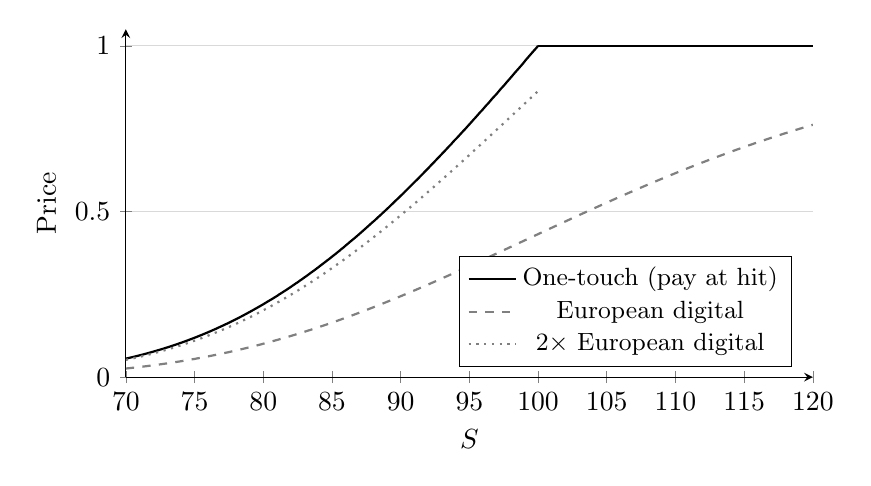
\begin{tikzpicture}
\begin{axis}[
    width=0.85\textwidth, height=6cm,
    xmin=70, xmax=120, ymin=0, ymax=1.05,
    xlabel={$S$}, ylabel={Price},
    ymajorgrids=true, grid style={gray!30},
    axis x line=bottom, axis y line=left,
    legend pos=south east, legend style={font=\small},
    samples=200,
    % Parameters: K = B = 100, tau = 1, r = 2%, q = 3%, sigma = 20%
    % mu = -0.75, lambda = 1.25
    declare function={
      Ncdf(\x) = 1/(1+exp(-0.07056*\x*\x*\x - 1.5976*\x));
      dtwo(\s) = (ln(\s/100) - 0.03)/0.2;
      zz(\s)   = ln(100/\s)/0.2 + 0.25;
      ot(\s)   = (100/\s)^0.5*Ncdf(-zz(\s)) + (100/\s)^(-2)*Ncdf(-zz(\s)+0.5);
    },
]
  \addplot[black, thick, domain=70:100] {ot(x)};
  \addlegendentry{One-touch (pay at hit)}
  \addplot[black, thick, domain=100:120, forget plot] {1};
  \addplot[gray, thick, dashed, domain=70:120] {exp(-0.02)*Ncdf(dtwo(x))};
  \addlegendentry{European digital}
  \addplot[gray, thick, dotted, domain=70:100] {2*exp(-0.02)*Ncdf(dtwo(x))};
  \addlegendentry{$2\times$ European digital}
\end{axis}
\end{tikzpicture}
\caption{Black--Scholes prices of a one-touch paying at hit and of a European
cash-or-nothing call ($Q=1$, $K=B=100$, $\tau=1$, $r=2\%$, $q=3\%$,
$\sigma=20\%$).}
\label{fig:bs-one-touch}
\end{figure}





% ==================================================================
\section{Pricing of Bermudan Digital Options}
\label{sec:bermudan}
% ==================================================================

This section prices digital options that can only be exercised on a finite set
of dates. As for American digitals, we first derive semi-closed-form prices
under the Black--Scholes model, and then price the options under the Heston
model calibrated in Section~\ref{sec:data}.




% ---------------------------------------------------------------------
\subsection{Black--Scholes Pricing}

A Bermudan cash-or-nothing call can only be exercised on a finite set of
observation dates $t < t_1 < \dots < t_m = T$. By the argument of
Proposition~\ref{prop:american-one-touch}, when $r \geq 0$ it is optimal to
exercise at the first observation date on which $S_{t_i} \geq K$. Writing
$s_i = t_i - t$, the price is
\begin{equation}
  V^{\mathrm{Berm}}_t = Q \sum_{i=1}^{m} e^{-r s_i}\,\bigl(F_{i-1} - F_i\bigr),
  \qquad F_0 = 1,
  \label{eq:bermudan-price}
\end{equation}
where
$F_i = \mathbb{Q}\left(S_{t_1} < K, \dots, S_{t_i} < K \mid \mathcal{F}_t\right)$
is the probability that the option has not been exercised after $i$
observations. Under~\eqref{eq:bs-sde}, $F_i$ is an $i$-dimensional normal
distribution function:
\begin{equation}
  F_i = \Phi_i\left(a_1, \dots, a_i;\, R_i\right),
  \qquad
  a_j = \frac{\ln(K/S_t) - \nu s_j}{\sigma\sqrt{s_j}},
  \qquad
  (R_i)_{jl} = \sqrt{\frac{s_{\min(j,l)}}{s_{\max(j,l)}}}.
  \label{eq:bermudan-cdf}
\end{equation}
For $m=1$, \eqref{eq:bermudan-price} reduces to the European
price~\eqref{eq:cash-call}. For a moderate number of dates, as for the annual
observations of an autocall, the multivariate normal distribution can be
evaluated numerically. For frequent monitoring, Monte Carlo simulation or the
continuity correction of Broadie, Glasserman and Kou~\cite{BroadieGlassermanKou1997}
is preferred: with equally spaced dates $\Delta t$ apart, the Bermudan digital
is approximated by the one-touch~\eqref{eq:one-touch-hit} with the barrier
shifted away from the spot,
\begin{equation}
  B^{\star} = K\,e^{-\eta\,\beta\,\sigma\sqrt{\Delta t}},
  \qquad
  \beta = -\frac{\zeta(1/2)}{\sqrt{2\pi}} \approx 0.5826,
  \label{eq:bgk}
\end{equation}
where $\zeta$ is the Riemann zeta function.

Since a Bermudan digital whose last date is $T$ can be exercised whenever the
European digital pays, and at least as early, the three exercise styles are
ordered for $r \geq 0$:
\begin{equation}
  D^{c} \;\leq\; V^{\mathrm{Berm}} \;\leq\; V^{\mathrm{Am}}.
  \label{eq:ordering}
\end{equation}
The observation frequency therefore interpolates continuously between the
European and the American digital.

% ---------------------------------------------------------------------
\subsection{Pricing under the Heston Model}
\label{subsec:heston-bermudan}

We now consider a digital with a bermudan style of exercise, the holder can exercise on a set of dates $t_1 < \dots < t_n = T$ and receive the payoff at the exercise date. 




% ==================================================================
\section{Greeks}
\label{sec:greeks}
% ==================================================================

% ==================================================================
\section{Hedging of a Digital}
\label{sec:hedging}
% ==================================================================

As shown in Section~\ref{subsec:call-spread}, a digital option can be hedged
and priced with a call spread. The remaining question is: which call spread?

% ==================================================================
\clearpage
\begin{thebibliography}{99}

\bibitem{Albrecher2007}
H.~Albrecher, P.~Mayer, W.~Schoutens and J.~Tistaert,
The Little Heston Trap,
\emph{Wilmott Magazine}, January:83--92, 2007.

\bibitem{BlackScholes1973}
F.~Black and M.~Scholes,
The Pricing of Options and Corporate Liabilities,
\emph{Journal of Political Economy}, 81(3):637--654, 1973.

\bibitem{BroadieGlassermanKou1997}
M.~Broadie, P.~Glasserman and S.~Kou,
A Continuity Correction for Discrete Barrier Options,
\emph{Mathematical Finance}, 7(4):325--349, 1997.

\bibitem{Bouzoubaa2010}
M.~Bouzoubaa and A.~Osseiran,
\emph{Exotic Options and Hybrids: A Guide to Structuring, Pricing and Trading},
Wiley, 2010.
\url{https://www.academia.edu/40236904/Exotic_Options_And_Hybrids_1_}

\bibitem{Gatheral2006}
J.~Gatheral,
\emph{The Volatility Surface: A Practitioner's Guide},
Wiley, 2006.

\bibitem{Haug2007}
E.~G.~Haug,
\emph{The Complete Guide to Option Pricing Formulas}, 2nd edition,
McGraw-Hill, 2007.

\bibitem{Heston1993}
S.~L.~Heston,
A Closed-Form Solution for Options with Stochastic Volatility with
Applications to Bond and Currency Options,
\emph{Review of Financial Studies}, 6(2):327--343, 1993.

\bibitem{Lewis2001}
A.~L.~Lewis,
A Simple Option Formula for General Jump-Diffusion and Other Exponential
L\'evy Processes, 2001.
\url{https://ssrn.com/abstract=282110}

\bibitem{LongstaffSchwartz2001}
F.~A.~Longstaff and E.~S.~Schwartz,
Valuing American Options by Simulation: A Simple Least-Squares Approach,
\emph{Review of Financial Studies}, 14(1):113--147, 2001.

\bibitem{Lord2010}
R.~Lord, R.~Koekkoek and D.~van~Dijk,
A Comparison of Biased Simulation Schemes for Stochastic Volatility Models,
\emph{Quantitative Finance}, 10(2):177--194, 2010.

\bibitem{Merton1973}
R.~C.~Merton,
Theory of Rational Option Pricing,
\emph{Bell Journal of Economics and Management Science}, 4(1):141--183, 1973.

\bibitem{ReinerRubinstein1991}
E.~Reiner and M.~Rubinstein,
Unscrambling the Binary Code,
\emph{Risk}, 4(9):75--83, 1991.

\bibitem{Shreve2004}
S.~E.~Shreve,
\emph{Stochastic Calculus for Finance II: Continuous-Time Models},
Springer, 2004.

\end{thebibliography}

\end{document}
